\\ \solution:
\begin{enumerate}
 \item The direction vector of $AD$ is 
\begin{align}
	\vec{m} = \vec{D}- \vec{A}
&=\myvec{\frac{-7}{2}\\\frac{1}{2}} - \myvec{1\\-1}
	=\frac{1}{2}\myvec{-9\\3} \equiv \myvec{-3 \\ 1}
	\\
	\implies  \vec{n} &=\myvec{1 \\ 3}
\end{align}
Hence the normal equation of median $AD$ is 
\begin{align}
\vec{n}^{\top}\myvec{\vec{x}-\vec{A}}&=0\\
\implies    \myvec{1 & 3}\vec{x}&=\myvec{1 & 3}\myvec{1\\-1}
    =-2
	\label{eq:median-ad}
\end{align}
\item For $BE$,
\begin{align}
	\vec{m}= \vec{E}- \vec{B}&=\myvec{-1\\-3} - \myvec{-4\\6}
       =\myvec{3\\-9}
       \equiv \myvec{1\\-3}
       \\
\implies 	
\vec{n} &= 
         \myvec{3\\1}
\end{align}
Hence the normal equation of median $BE$ is 
\begin{align}
\vec{n}^{\top}\myvec{\vec{x}-\vec{B}}&=0\\
\implies
	\myvec{3 & 1}   \vec{x}&=\myvec{3 &1}\myvec{-4\\6}
    =-6
	\label{eq:median-be}
\end{align}
\item For median $CF$,
\begin{align}
	\vec{m} = \vec{F}- \vec{C} &=
\myvec{\frac{-3}{2}\\\frac{5}{2}} - \myvec{-3\\-5}
       =\myvec{\frac{3}{2}\\\frac{15}{2}}
       \equiv \myvec{1 \\ 5}
       \\
	\implies \vec{n} &=\myvec{5 \\ -1}
\end{align}
Hence the normal equation of median $CF$ is 
\begin{align}
\vec{n}^{\top}\myvec{\vec{x}-\vec{C}}&=0\\
	\implies \myvec{5 & -1}\vec{x}&=\myvec{5 & -1}\myvec{-3\\-5}
    =-10
	\label{eq:median-cf}
\end{align}
\end{enumerate}
\iffalse
\begin{figure}
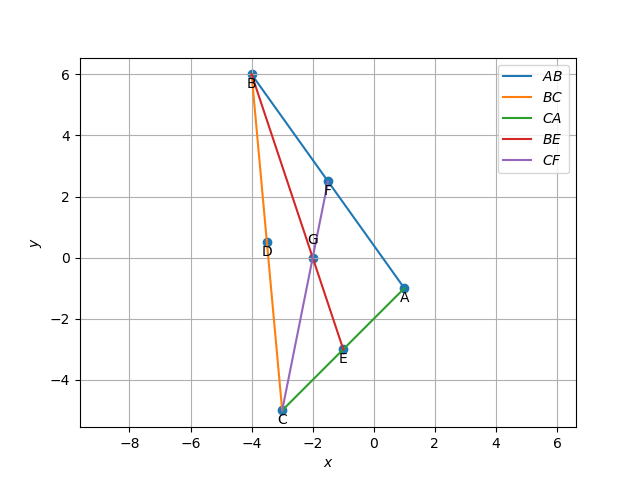
\includegraphics [width=\columnwidth] {solutions/1/2/2/figs/figure.png}
\caption{ Medians $AD$ , $BE$ and $CF$}
\label{fig: medians}
\end{figure}
\fi



